\subsection{High compartmentalization and disparity around gastrulation}
%objective
I estimated the degree of compartmentalization calculating the relative area of expression of hundreds of genes during development.
My intention here was not to focus on individual genes, but to get a global overview of the embryo compartmentalization and differentiation processes.

%results
The results showed a non-linear decrease in the mean relative area of expression (an inverted saturation curve), with the major decrease occurring at very early development, from maternal to early gastrula stage (Fig. \ref{fig:Art-I-3measures}).
Practically half of the genes in follows this decrease pattern: 46\% of the genes were characterized as having a non-linear decrease in their relative area.
The results show that the disparity increases non-linearly, again with the major change in the early stages.
%
It is important to notice that these should not be necessarily the case, as the disparity relates to how different genetically are the different regions of the embryo in different stages, so it could be that between two stages the relative area of expression decreases but not the disparity if the genes are expressed in the same part of the embryo.

%discussion

These results are consistent with the hypothesis that the Drosophila embryo becomes compartmentalized in a progressively more fine-grained manner over developmental time. 
More importantly, they show that this process happens quite early in Drosophila, i.e., around gastrulation.
This is, most genes start being expressed in broad areas of the embryo and over time their expression becomes progressively restricted into smaller and smaller spatial domains.

This earlier compartmentalization probably is due to Drosophila's derived early development, namely, the syncytial blastoderm. During this stage, approximately 4,000 cell nuclei can `communicate' with each other only by TFs \citep{Jaeger2011}. The direct cross regulation of gene expression facilitates a rapid and highly dynamic process which seems to be responsible for the early spatial restriction of a great proportion of developmental genes.

%%%%%%%%%%%%%%%%%%%%%%%%%%%%%%%%%%%%%%%%%%%%%%%%%%%%%%%%%%%%%%%%%%%%%%%%%%%%%%%%%%%%% 
\begin{figure}[h]
  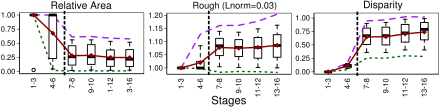
\includegraphics[width=\textwidth]{./Images/Art-I/3_measures.png}
  \centering
  \caption{Distribution plot of the relative area of expression (left), roughness (center) and disparity (right) for all genes in each stage. Diamonds represent the mean, boxes the IQR. Whiskers 10 and 90 percentiles. Dashed line represents the max values and dotted line the min values (mean of the last and first decile, respectively). Stages on the x-axis, vertical dashed line represents gastrulation entry.}
  \label{fig:Art-I-3measures}
\end{figure}
%%%%%%%%%%%%%%%%%%%%%%%%%%%%%%%%%%%%%%%%%%%%%%%%%%%%%%%%%%%%%%%%%%%%%%%%%%%%%%%%%%%%% 

\subsection{The leading role of TFs and GFs}

%objective
Then, I wanted the test if the hypothesis transcription factors (TFs) and growth factors (GFs) have a a leading role in pattern formation and compartmentalization.
%results 1
The TFs (GO:0003700) and GFs (GO:0008083) showed smaller relative area of expression that the rest of genes in the blastoderm stage (Fig. \ref{fig:Art-I-3measures}).
	\nomenclature{GF}{Growth Factor}
	\nomenclature{KW}{Kruskal-Wallis test}
%
The TFs are also expressed in smaller areas than the rest of the genes in all subsequent stages, while the GFs are expressed in smaller areas at the blastoderm (stage 4-6) and extended germ band stages (stage 9-10 and 11-12) (I, Fig.4).

%discussion 1
These results are complementary to the study done by \citet{Hammonds2013}, who made an extensive analysis of TFs expression using the BDGP database, using manual annotation of gene expression based on an anatomical controlled vocabulary and classifying every gene as ubiquitous, patterned, ubiquitous-patterned, or maternal. 
They found that the fraction of TFs expressed in a restricted pattern (assigned to a tissue) was higher, when compared to other genes, in all zygotic stages with the exception of the stage 13-16. 

The results I show for stages 4-6, 7-8, 9-10 and 11-12 are consistent with Hammonds et al., as the higher proportion of the TF genes showing a restricted or tissue-specific expression pattern would imply that TFs are expressed in smaller areas in the embryo. For the 13-16 stage, contrary to these authors, I showed that the TFs are highly compartmentalized. This might indicate a limitation of the annotation method used by Hammonds et al., to capture the high spatial compartmentalization of the TFs in this stage.

In general, these results support the hypothesis of the leading role of TFs and GFs in driving pattern formation and compartmentalization in the early embryo.

%results & discusion 2
In the blastoderm stage the disparity of the regions based only on the TFs is much greater than the one based on all the genes ((KW pvalue $<0.001$; Fig. \ref{fig:Art-I-3measures}) indicating that these genes account for a large portion of the diversity of gene expression patterns.

In general, the fact that TF genes have lower relative area (i.e., are more compartmentalized) than the rest of the genes, especially in the stage before entering gastrulation, is consistent with the leading role of these genes in driving pattern formation and the resulting compartmentalization of the embryo.

%%%%%%%%%%%%%%%%%%%%%%%%%%%%%%%%%%%%%%%%%%%%%%%%%%%%%%%%%%%%%%%%%%%%%%%%%%%%%%%%%%%%% 
\subsection{Roughness increases non-linearly}
%objective
The roughness measure informs about the overall imbrication or convolution of the shape of a gene expression contour at different spatial scales, relative to a circular shape.
%results
Our results (Fig. \ref{fig:Art-I-3measures}) show that roughness increases in a non-linear way during development, and that the major increase is in the transition from the blastoderm to the early gastrula.
The maximal values (mean of the last decile) increase initially in the pre-gastrula, reach a stationary phase at mid-embryogenesis and finally increase in the last stages. 
As I mentioned in the literature review (section X), the maximal values are informative about the overall morphological spatial complexity of the embryo in a given stage.

When comparing roughness at different spatial scales (I, Methods), I found that in the last three stages the roughness values are significantly higher at smaller spatial scales is significantly higher that at the higher spatial scales.(Fig. S2 in article I). 
%discussion
This suggests that complexity may be increasing not only through all the development but also that it does at finer spatial scales over time.


%%%%%%%%%%%%%%%%%%%%%%%%%%%%%%%%%%%%%%%%%%%%%%%%%%%%%%%%%%%%%%%%%%%%%%%%%%%%%%%%%%%%% 
\subsection{Main spatio-temporal profiles of gene expression}
%objective
I performed a time series cluster analysis \citep{Ernst2006} using the relative area of expression in order to know which were the most common spatio-temporal profiles (I, Fig. 5).
%results
I found eight main spatio-temporal profiles, the most common following the global profile of non-linear decrease in the first stages (I, Fig 5)

Among the rest of profiles, I found both linear increase and decrease profiles and a `hill-like' profile (initial increase and further decrease with the higher values at stage 7-8)
%
The linear decrease profile (n=167 genes) was enriched with `mitotic cell cycle' (GO:0000278), `RNA processing' (GO:0006396) and `chromatin modification' (GO:0016568) GOterm genes, highlighting biological processes that first are present in the whole embryo and become more and more restricted in space as development proceeds.
%discussion
The `mitotic cell cycle' term, for example, most likely relates to the fast mitotic cycles in the earliest embryo. During stage 1-3 nine fast and synchronic mitotic divisions take place in the entire embryo, then in stage 4-6 mitotic divisions 10-13 occur more slowly, almost synchronically. The 14th cycle, zygotically controlled, is long and of different durations in the embryo.

With a temporal co-expression cluster analysis using microarray data through the life cycle of \textit{D. melanogaster}, \citet{Arbeitman2002} found that most cell cycle genes were expressed at high levels during the first 12h, but only a few are expressed at high level thereafter.
My analysis is consistent with this, as I found that the profile of linear decrease (I, Fig. 5A) is enriched with such genes. In this sense, this study is complementary to Arbeitman et al., and adds the spatial dimension to their temporal expression profiles.


%%%%%%%%%%%%%%%%%%%%%%%%%%%%%%%%%%%%%%%%%%%%%%%%%%%%%%%%%%%%%%%%%%%%%%%%%%%%%%%%%%%%% 
\subsection{Gene synexpression territories in the embryo}
%objective
Finally, using a clustering algorithm, I made a dendrogram representing the relative degrees of similarities between all regions of all the stages at the same time (Fig. \ref{fig:Art-I-territories} A).
After cutting the dendrogram at a certain level and choosing only territories with at least 50 genes expressed with a minimum specificity (see methods in I for a detailed description), I ended up with 30 clusters (Fig. \ref{fig:Art-I-territories} B), which I will call `synexpression territories' (ST) from now on.
	\nomenclature{ST}{Synexpression territories}
I grouped the STs in eight `meta-territories' to analyse how the different STs relate between them.

%results
The results show that stages 1-3 and 4-6 each one form a ST. If a cut-off is selected so that stage 4-6 is divided in four sub-territories (I,Fig. S3) the embryo splits in four parts: anterior, posterior, dorsal and ventral.
This correspond to a nearly Cartesian system one could expect from the two signalling systems known in the earliest patterning in Drosophila (the A/V and D/V signalling cascades; \citep{Gilbert2014}).
%
The STs seem to coincide with the known embryo fatemap (see Fig. \ref{fig:Art-I-territories} D; \citealp{Hartenstein1993}) and many of them are enriched with GOterms that coincide with their expected fate.
For example, in stage 7-8 (just after gastrulation) there is a ST that corresponds spatially with the germband and is enriched with mesodermal GOterms (Fig. Fig. \ref{fig:Art-I-territories} C).

There are two meta-territories that appear in the last stage (light blue and green, Fig. \ref{fig:Art-I-territories} C), which suggests that the tissues/organs related to those STs differentiate quite late.
%
%% discussion
One is enriched with terms related to epidermis such as cuticle development (`chitin catabolic process' [GO:0006032] and `cuticle development' [GO:0042335] synexpression territories 33 and 38), which coincides with cuticle deposition by epithelial cells during stage 16 \citep{Ostrowski2002}.
%
The other corresponds spatially with the CNS of the embryo and is indeed enriched with CNS GO-terms
The CNS territory is enriched with GOterms like `dendrite morphogenesis' (GO:0048813) and `axon guidance' (GO:0007411). 
	\nomenclature{CNS}{Central Nervous System}

\begin{figure}[h]
  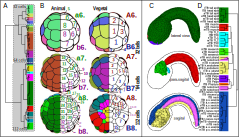
\includegraphics[width=0.65\textwidth]{./Images/Art-I/territories.png}
  \centering
  \caption{Synexpression territories (ST). (A) Dendrogram produced by hierarchical clustering on a similarity matrix (pearson's correlation) of all the embryo regions of the six stages. Red line shows the cut-off to produce 40 STs. (B) Dendrogram reconstructed using only territories with at least 50 genes with a minimum specificity (I, methods). The coloured boxes show the main branches of the dendrogram. The number indicated inside the boxes represent the stages each ST corresponds to (3 is stage 7-8, 4 is stage 9-10, 5 is stage 11-12 and 6 is stage 13-16). The ST number is at the right. (C) STs mapped onto the embryo. Gray regions have less than 50 genes expressed. Background color refers to which `meta-territory' (in B) each ST is part of. Coloured circles represent GOterm enrichment of a specific tissue/germ layer derivative (shown in E). Stages in the lower-left part of each embryo. From stage 7-8, the ST number (as in B) is indicated. (D) Hartenstein's embryo schemes \citep{Hartenstein1993} with their respective stages in the left upper part. (E) Colour code of specific tissue/germ layer derivative used in C.)}
  \label{fig:Art-I-territories}
\end{figure}

In summary, the STs and their spatial distribution largely reconstruct the known compartmentalization of the embryo. First A/P and D/V compartments are formed (stage 3-4), later germ-band, non-germ-band and posterior midgut compartments (stage 7-8), the germ-band then splits into foregut, hindgut and rest of mesoderm while the nervous system starts to differentiate (stage 9-10) and finally the midgut territories arise (stage 11-12).
Therefore, this specific sequence resembles the expected one based on changes in embryonic anatomy and fate maps collected over many years and analysed qualitative (Hartenstein, 1993). 
Thus, my study reinforce this compartmentalization time line using the spatio-temporal expression of hundreds of genes.

%%%%%%%%%%%%%%%%%%%%%%%%%%%%%%%%%%%%%%%%%%%%%%%%%%%%%%%%%%%%%%%%%%%%%%%%%%%%%%%%%%%%% 